\documentclass[aspectratio=169,12pt,spanish]{beamer}
\usepackage[T1]{fontenc}
\usepackage[spanish]{babel}

\usepackage{wrapfig}

%\usepackage{multicol}
%\usepackage{mathtools}

\usepackage[normalem]{ulem}

\usepackage{pgf,tikz}
\usetikzlibrary{matrix}
\usetikzlibrary{arrows}

%\usepackage{wrapfig}
\mode<presentation>
\usefonttheme{professionalfonts}
\usetheme{Darmstadt}
\usecolortheme{orchid}
\useoutertheme{default}
\setbeamertemplate{headline}{}

\newcounter{savedenum}
\newcommand*{\saveenum}{\setcounter{savedenum}{\theenumi}}
\newcommand*{\resume}{\setcounter{enumi}{\thesavedenum}}

\renewcommand{\baselinestretch}{1.1}

%gets rid of bottom navigation bars
\setbeamertemplate{footline}[page number]

%gets rid of navigation symbols
\setbeamertemplate{navigation symbols}{}

%\frameframe{none} % No default frame

%\setlength{\framewidth}{8.7in} \setlength{\frameheight}{7.2in}

\parindent 0pt
\setlength{\parskip} {1ex plus 0.5ex minus 0.2ex}


\usepackage[bbgreekl]{mathbbol}
\usepackage{amssymb, amsthm, amsmath}
\usepackage{bm}

\newtheorem{ejercicio}{Ejercicio}
\newtheorem{proposition}[theorem]{Proposición}

\DeclareSymbolFontAlphabet{\mathbb}{AMSb}
\DeclareSymbolFontAlphabet{\mathbbl}{bbold}

\usepackage{multicol}
\usepackage{colortbl}
\usepackage{lmodern}
\usepackage{tabularx}
\usepackage{multirow}
\usepackage{stmaryrd}
\usepackage{color}
\usepackage{graphicx}
\usepackage{hyperref}

\graphicspath{ {../../images} }
\usepackage{listings}
\lstset{
  basicstyle=\ttfamily,
  columns=fullflexible,
}

\usepackage{url}
\usepackage{multicol}
\usepackage{dsfont}

% Bold symbols for vectors and matrices
\newcommand{\xstar}{\bm{x}^{\star}}
\newcommand{\alphab}{\bm{\alpha}}
\newcommand{\ab}{\bm{a}}
\newcommand{\bb}{\bm{b}}
\newcommand{\cb}{\bm{c}}
\newcommand{\db}{\bm{d}}
\newcommand{\eb}{\bm{e}}
\newcommand{\gb}{\bm{g}}
\newcommand{\mb}{\bm{m}}
\newcommand{\pb}{\bm{p}}
\newcommand{\qb}{\bm{q}}
\newcommand{\rb}{\bm{r}}
\newcommand{\ssb}{\bm{s}}
\newcommand{\ub}{\bm{u}}
\newcommand{\vb}{\bm{v}}
\newcommand{\wb}{\bm{w}}
\newcommand{\xb}{\bm{x}}
\newcommand{\yb}{\bm{y}}
\newcommand{\zb}{\bm{z}}

\newcommand{\Ab}{\bm{A}}
\newcommand{\Bb}{\bm{B}}
\newcommand{\Cb}{\bm{C}}
\newcommand{\Db}{\bm{D}}
\newcommand{\Eb}{\bm{E}}
\newcommand{\Fb}{\bm{F}}
\newcommand{\Gb}{\bm{G}}
\newcommand{\Hb}{\bm{H}}
\newcommand{\Ib}{\bm{I}}
\newcommand{\Id}{\bm{I}}
\newcommand{\Kb}{\bm{K}}
\newcommand{\Lb}{\bm{L}}
\newcommand{\Mb}{\bm{M}}
\newcommand{\Pb}{\bm{P}}
\newcommand{\Qb}{\bm{Q}}
\newcommand{\Rb}{\bm{R}}
\newcommand{\Sb}{\bm{S}}
\newcommand{\Tb}{\bm{T}}
\newcommand{\Ub}{\bm{U}}
\newcommand{\Vb}{\bm{V}}
\newcommand{\Wb}{\bm{W}}
\newcommand{\Xb}{\bm{X}}
\newcommand{\Yb}{\bm{Y}}
\newcommand{\Zb}{\bm{Z}}
\newcommand{\Lambdab}{\bm{\Lambda}}
\newcommand{\cero}{\bm{0}}

% Rings and fields
\newcommand{\A}{\mathbb{A}}
\newcommand{\Z}{\mathbb{Z}}
\newcommand{\Q}{\mathbb{Q}}
\newcommand{\C}{\mathbb{C}}
\newcommand{\R}{\mathbb{R}}
\newcommand{\K}{\mathbb{K}}
\newcommand{\N}{\mathbb{N}}

\newcommand{\borel}{{\mathcal B}}
\newcommand{\pmom}{{\rho_{\text{mom}}}}
\newcommand{\MX}{{\mathcal{M}(X)}}


% Inner product
\newcommand{\innerl}[2]{\langle #1, #2 \rangle}
\newcommand{\inner}[2]{#1 \boldsymbol{\cdot} #2}
\newcommand{\innerTrace}[2]{#1 \bullet #2}

% Symmetric and positive definite matrices
\newcommand{\Splusplusn}{{\mathcal S_{++}^n}}
\newcommand{\Splusn}{{\mathcal S_+^n}}
\newcommand{\Splus}{{\mathcal S_+}}
\newcommand{\Sym}{{\mathcal S}}
\newcommand{\Symn}{{\mathcal S^n}}

% Cones
\newcommand\CC{\mathcal{C}}
\DeclareMathOperator{\cone}{cono}
\DeclareMathOperator{\conv}{conv}
\DeclareMathOperator{\supp}{supp}


% Spectrahedron
\newcommand{\eLL}{{\mathcal L}}

% Matrices and vectors over R or C
\newcommand{\Rnn}{\R^{n\times n}}
\newcommand{\Cnn}{\C^{n\times n}}
\newcommand{\Rn}{\R^{n}}
\newcommand{\Rm}{\R^{m}}


% Math operators
\DeclareMathOperator{\Tr}{Tr}
\DeclareMathOperator{\tr}{Tr}
\DeclareMathOperator{\interior}{int}
\DeclareMathOperator{\rank}{rank}
\DeclareMathOperator{\diag}{diag}

\newcommand\one{\mathds{1}} 

\pagestyle{empty}

\begin{document}

%------------------------------------------------------------------

\begin{frame}

 \begin{center}

\Large\textbf{Optimización Semidefinida} \\
\large\textbf{Clase 14 - Optimización polinomial}
%\vspace{0.5cm}

% \textit{Santiago Laplagne} \\
%slaplagn@dm.uba.ar \\


%\vspace{0.5cm}
%{\small Trabajo en progreso en conjunto con \emph{Jose Capco} (Universit\"at Innsbruck) y \emph{Claus Scheiderer} %(Universit\"at Konstanz).} \\

\vspace{1cm}
 Segundo Cuatrimestre 2021
 \\
 {\small Facultad de Ciencias Exactas y Naturales, UBA}
 \end{center}

\end{frame}


%------------------------------------------------------------------


\begin{frame}

\frametitle{Aplicación: optimización polinomial sin restricciones}

Vimos que podemos plantear el problema de encontrar el mínimo $\gamma$ de un polinomio como un problema de optimización
\begin{alignat*}{2}
  & \text{maximizar: } & & \gamma  \\
  & \text{sujeto a: } & \quad & p(\xb) - \gamma \ge 0 \ \forall \xb \in \R^n.
\end{alignat*}

Si restringimos el conjunto factible a sumas de cuadrados:
\begin{alignat*}{2}
  & \text{maximizar: } & & \gamma  \\
  & \text{sujeto a: } & \quad & p(\xb) - \gamma \quad \text{es SOS}.
\end{alignat*}
obtenemos en general una cota inferior
$$
p_{SOS} \le p_{\star}.
$$
\end{frame}

%------------------------------------------------------------------

\begin{frame}

\frametitle{El problema 17 de Hilbert}

¿Cómo podemos mejorar la cota relajando las restricciones?

En 1900, Hilbert publicó una lista de 23 problemas abiertos que resultaron muy influyentes en el desarrollo de la matemática del siglo XX.

\begin{theorem}{Problema 17 de Hilbert, 1900.}
Sea $f \in \R[X_1, \dots, X_n]$, si $f \ge 0$ para todo $(x_1, \dots, x_n) \in \R^n$, entonces
\[
f = \left(\frac{p_1}{q_1}\right)^2 + \dots + \left(\frac{p_s}{q_s}\right)^2,
\]
$p_i, q_i \in \R[X_1, \dots, X_n]$.
\end{theorem}

El teorema fue demostrado por Artin en 1923.


\end{frame}

%------------------------------------------------------------------

\begin{frame}

\frametitle{Ejemplo}

Para el polinomio de Motzkin
$$
M(x,y) = x^4y^2 + x^2 y^4 + 1 - 3x^2y^2,
$$
multiplicandolo por $x^2 + y^2$ (que es obviamente positivo) obtenemos la descomposición
$$
(x^2+y^2) M(x,y) = y^2(1-x^2)^2 + x^2(1-y^2)^2 + x^2y^2(x^2 + y^2-2)^2,
$$
que da un certificado de la positividad de $M(x,y)$.


\end{frame}

%------------------------------------------------------------------

\begin{frame}

\frametitle{Relajaciones de Parrilo}

En base al teorema de Artin, deducimos
$$
f(\xb) \ge 0 \ \forall \xb \in \R^n \quad \iff \quad \exists p, q \text{ SOS tales que } qf = p.
$$

Intentamos plantear el problema como un problema SDP:
\begin{center}
Determinar si existen $\Qb_1, \Qb_2 \succeq 0$ tales que $(\vb_1^t \Qb_1 \vb_1) f = \vb_2^t \Qb_2 \vb_2$.
\end{center}
con $\vb_1$, $\vb_2$ los vectores de monomios de ciertos grados.

Observamos que la igualdad da restricciones lineales en los coeficientes de $\Qb_1$ y $\Qb_2$ y por lo tanto es un problema de factibilidad SDP.

Sin embargo, necesitamos conocer cotas para los grados de $q$ y $p$ para poder plantearlo de esta forma.

\end{frame}

%------------------------------------------------------------------

\begin{frame}

\frametitle{Relajaciones de Parrilo}

A diferencia del caso en que escribimos a $f$ como sumas de cuadrados, ahora no podemos deducir una cota directa para los grados de $p$ y $q$ a partir de la expresión $qf = p$.

Si $f$ tiene grado $e$ y fijamos el grado $d$ del denominador $q$ (y por lo tanto el grado de $p$ es $d + e$), obtenemos el problema de factibilidad
\begin{alignat*}{2}
  & \text{existencia: } & & p, q \in \R[\xb]  \\
  & \text{sujeto a: } & \quad & q f = p \\
  &&& \deg(q) < d, \\
  &&& \deg(p) < d + e.
\end{alignat*}
\end{frame}

%------------------------------------------------------------------

\begin{frame}

\frametitle{Relajaciones de Parrilo}

Planteamos el problema anterior como problema SDP
\begin{alignat*}{2}
  & \text{existencia: } & & \Qb_1, \Qb_2 \\
  & \text{sujeto a: } & \quad & (\vb_1^t \Qb_1 \vb_1) f = \vb_2^t \Qb_2 \vb_2 \\
  &&& \Qb_1, \Qb_2 \succeq 0
\end{alignat*}
para $\vb_1$, $\vb_2$ los vectores de monomios de grados $d$ y $d+e$ respectivamente y $\Qb_1, \Qb_2$ de los tamaños apropiados.

Tomando $d$ suficientemente grande, este problema es equivalente al problema original de determinar si $f(\xb)$ es positivo.

Pero ¿qué tan grande debemos tomar $d$?
\end{frame}

%------------------------------------------------------------------

\begin{frame}

\frametitle{Cotas para el teorema 17 de Hilbert}

{\footnotesize
\textbf{An elementary recursive bound for effective Positivstellensatz and Hilbert 17-th problem}

Henri Lombardi, Daniel Perrucci, Marie-Françoise Roy

We prove an elementary recursive bound on the degrees for Hilbert 17-th problem. More
precisely we express a nonnegative polynomial as a sum of squares of rational functions, and
we obtain as degree estimates for the numerators and denominators the following tower of
five exponentials
$$2^{2^{d^{4^k}}}$$
where $d$ is the degree and $k$ is the number of variables of the input polynomial.
}

\vspace{0.5cm}

Esta cota no es útil en la práctica.

\end{frame}


%------------------------------------------------------------------

\begin{frame}

\frametitle{Optimización polinomial}

Consideramos ahora el problema de hallar el mínimo de un polinomio $f$ de grado $e$ en $\R^n$.

Análogamente al caso de sumas de cuadrados, planteamos el problema
\begin{alignat*}{2}
  & \text{maximizar: } & & \gamma  \\
  & \text{sujeto a: } & \quad & q(\xb) (f(\xb) - \gamma) =  p(\xb) \\
  &&& p, q \quad \text{SOS}.
\end{alignat*}

\end{frame}


%------------------------------------------------------------------

\begin{frame}

\frametitle{Optimización polinomial}

En este caso, para poder resolver el problema mediante un programa SDP necesitamos fijar el grado de los polinomios $p$ y $q$. Obtenemos el problema
\begin{alignat*}{2}
  & \text{maximizar: } & & \gamma  \\
  & \text{sujeto a: } & \quad & q(\xb) (f(\xb) - \gamma) =  p(\xb) \\
  &&& p, q \quad \text{SOS}, \\
  &&& \deg(q) < d, \deg(p) < d + e.
\end{alignat*}

Si tomamos una sucesión creciente de grados $d_1 < d_2 < d_3 < ...$ obtenemos
$$
\gamma^{\star}_{d_1} \le \gamma^{\star}_{d_2} \le \gamma^{\star}_{d_3} \le \dots \le f^{\star}
$$
y tomando $d$ suficientemente grande vamos a encontrar el óptimo de $f$.


\end{frame}


%------------------------------------------------------------------

\begin{frame}

\frametitle{Espacio publicitario}

Más generalmente, Parrilo usa el teorema de positividad de Stengle:

\begin{center}
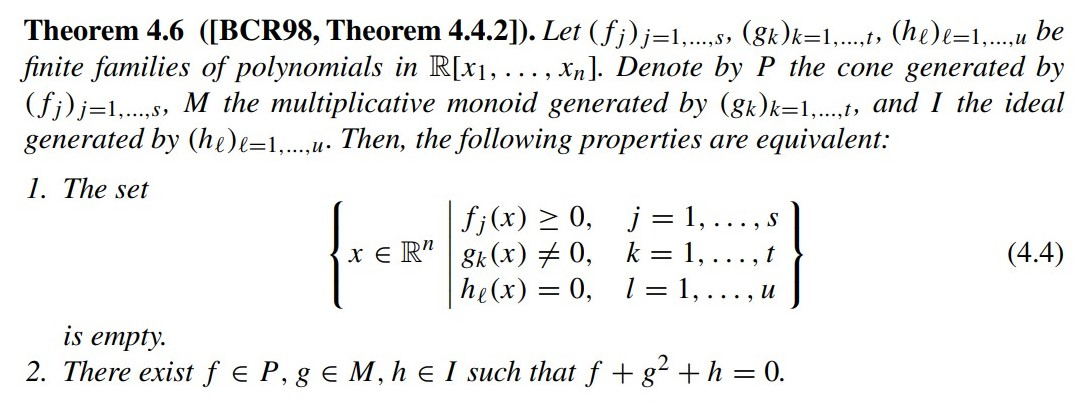
\includegraphics[scale=.4]{sos_stengle.jpg}
\end{center}
Para saber más sobre teoremas de positividad, cursar la materia ``Polinomios positivos y sumas de cuadrados'' que dicta Daniel Perrucci.


\end{frame}


%------------------------------------------------------------------

\begin{frame}

\frametitle{Optimización sobre conjuntos semi-algebraicos}

Un conjunto semi-algebraico básico en $\R^n$ es un conjunto $S$ definido por desigualdades polinomiales
$$
S = \{\xb \in \R^n \mid g_1(\xb) \ge 0, \dots, g_m(\xb) \ge 0\}
$$
para polinomios $g_1, \dots, g_m \in \R[\xb]$.

Consideramos el problema de minimizar un polinomio $f \in \R[\xb]$ en $S$ en el caso en que $S$ es compacto.



\end{frame}

%------------------------------------------------------------------

\begin{frame}

\frametitle{Módulos cuadráticos}

Llamamos $\R[\xb]^2$ al conjunto de todos los cuadrados $p^2$ de polinomios $p \in \R[\xb]$.

Llamamos $\Sigma\R[\xb]^2$ al conjunto de todos los polinomios sumas de cuadrados.

Llamamos $\Sigma\R[\xb]^2 g_i$ al conjunto de todas las sumas de polinomios en $p g_i$ con $p \in \Sigma\R[\xb]^2$.

Definimos el módulo cuadrático generado por $g_1, \dots, g_m$ como el conjunto
\begin{align*}
M &= \Sigma + \Sigma\R[\xb]^2 g_1 + \cdots +  \Sigma\R[\xb]^2 g_m \\
&= \left\{ \sum_{i=0}^m \sigma_i g_i \mid \sigma_i \in \Sigma\R[\xb]^2 \right\} \subset \R[\xb],
\end{align*}
tomando $g_0 = 1$.



\end{frame}

%------------------------------------------------------------------

\begin{frame}

\frametitle{Módulos cuadráticos}

Para $M = \Sigma\R[\xb]^2 + \Sigma\R[\xb]^2 g_1 + \cdots +  \Sigma\R[\xb]^2 g_m$, es inmediato:

$$
p \in M \quad \Rightarrow  \quad p(\xb) \ge 0 \ \forall \xb \in S.
$$

Para obtener un resultado recíproco, hacemos la siguiente definición.

\begin{definition}
Decimos que un módulo cuadrático $M$ es arquimedeano si
\begin{align}
\label{compacto}
\exists N \in \N \text{ tal que } N - \sum_{i=1}^n X_i^2 \in M.
\end{align}
\end{definition}


\end{frame}

%------------------------------------------------------------------

\begin{frame}

\frametitle{Ejemplo 6.3.1 Positive Polynomials, A. Prestel \& C. Delzell}
Consideramos los polinomios en $\R[x,y]$:
$$
g_1(x,y) = x - \frac{1}{2}, \quad g_2(x,y) = y - \frac{1}{2}, \quad g_3 = 1-xy.
$$

\begin{minipage}{0.45\textwidth}
El conjunto
$$S = \{(x,y) \mid g_i(x,y) \ge 0, i = 1, 2, 3 \}$$ cuyo gráfico vemos en la figura es compacto.
\end{minipage}\hfill
\begin{minipage}{0.45\textwidth}
\begin{center}
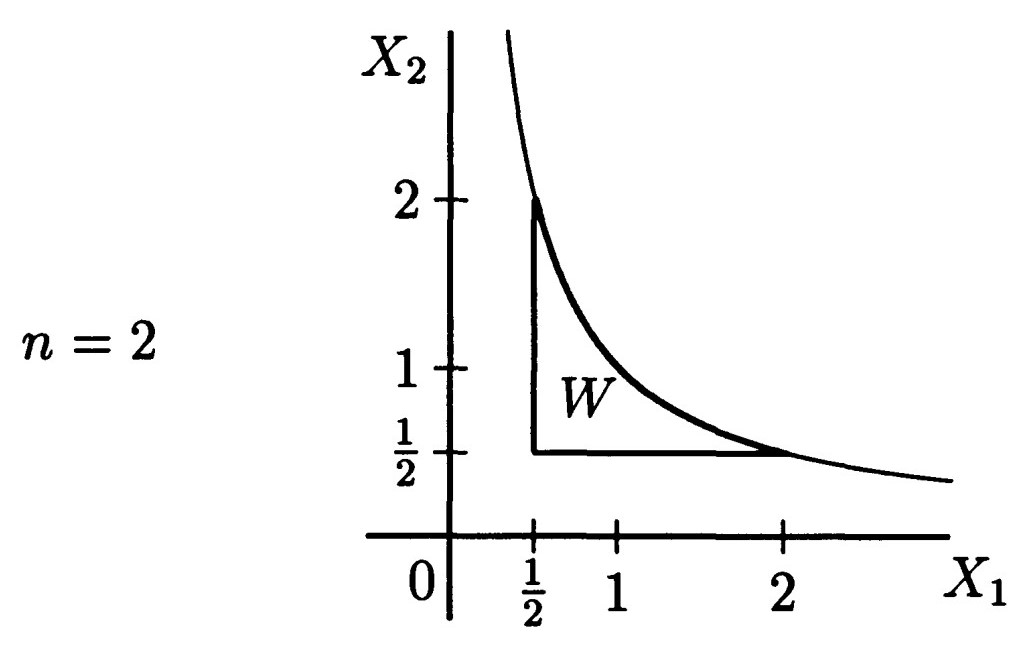
\includegraphics[scale=.18]{sos-noarquimedeano.jpg}
\end{center}
\end{minipage}

Sin embargo el módulo cuadrático
$$
M = \{a + b (x - \frac{1}{2}) + c (x-\frac{1}{2}) + d (1 - xy) \}
$$
con $a,b,c,d \in \Sigma\R[\xb]^2$ no es arquimedeano.
\end{frame}

%------------------------------------------------------------------

\begin{frame}

\frametitle{Módulos cuadráticos arquimedeanos}

Son equivalentes

\begin{enumerate}
\item $M$ es arquimedeano.
\item Existe $p \in M$ tal que $\{x \in \R^n \mid p(\xb) \ge 0\}$ es compacto.
\end{enumerate}

\end{frame}

%------------------------------------------------------------------

\begin{frame}

\frametitle{Módulos cuadráticos}
Obtenemos el siguiente teorema de positividad:

\begin{theorem}[Putinar positivstellensatz]
Si $S$ es un conjunto semi-algebraico básico compacto y $M$ es arquimedeano,
$$p \in \R[\xb] \text{ satisface  } p > 0 \text{ en } S \Rightarrow p \in M.$$
\end{theorem}

Observamos que este teorema solo caracteriza a los polinomios estrictamente positivos y no a los no--negativos.

\end{frame}

%------------------------------------------------------------------

\begin{frame}

\frametitle{Ejemplo justo antes de Lema 8.2.3 (DP)}

Consideramos $f = 1 - x^2$ y $h = (1-x^2)^3$.

Definimos $S = \{ x \in \R \mid h(x) \ge 0\} = [-1, 1]$ y vemos que $f \ge 0$ en $S$.

Sin embargo, no existen $\sigma_0, \sigma_1$ SOS tales que
$$
f = \sigma_0 + \sigma_1 h.
$$

\end{frame}

%------------------------------------------------------------------

\begin{frame}

\frametitle{Relajación SDP}
Para el problema de optimización de un polinomio $f$ sobre $S$ obtenemos
$$
f^{\star} = \sup\{a \in \R \mid f - a \in M\}.
$$

En base al ejemplo anterior, este supremo podría no alcanzarse.

Como en los problemas anteriores, no podemos plantear la condición $f - a \in M$ debido a que no tenemos una cota para los coeficientes sumas de cuadrados que pueden aparecer en la escritura
$$
f - a = p_0 + p_1 g_1 + \cdots + p_m g_m.
$$

\end{frame}

%------------------------------------------------------------------

\begin{frame}

\frametitle{Relajación SDP}
Introducimos entonces para $k \in \N$ aproximaciones $M_k \subset \R[\xb]_k$ de $M$:
\begin{align*}
M_k &= \Sigma\R[\xb]^2_{d_0} + \Sigma\R[\xb]^2_{d_1} g_1 + \cdots +  \Sigma\R[\xb]^2_{d_m} g_m \\
&= \left\{ \sum_{i=0}^m \sigma_i g_i \mid \sigma_i \in \Sigma\R[\xb]^2, \deg(\sigma_i g_i) \le k \right\} \subset \R[\xb],
\end{align*}
donde $d_i = \max\{d \in \N \mid 2d + \deg g_i \le k\}$.

Observamos que la cota sobre los grados se aplica sobre todos los polinomios que aparecen en la descomposición y no solo sobre el polinomio resultante.

No debemos confundir $M_k$ con $M \cap \R[\xb]_k \supset M_k$.

\end{frame}

%------------------------------------------------------------------

\begin{frame}

\frametitle{Relajación SDP}


Obtenemos el siguiente problema SDP
\begin{alignat*}{2}
  & \text{maximizar: } & & \gamma  \\
  & \text{sujeto a: } & \quad & f - \gamma \in M_k.
\end{alignat*}

Para todo $k$ se cumple $\gamma_k^{\star} \le f^{\star}$ e incrementando el valor de $k$ obtenemos una secuencia creciente
$$(\gamma_k^{\star})_{k \in \N}$$
que converge a $f^{\star}$.



\end{frame}

%-----------------------------------

\end{document} 